\section{Operazioni fra insiemi}

\subsection{Intersezione di insiemi}
L'intersezione di due insiemi si scrive S $\cap$ T,
L'insieme risultante contiene tutti e soli gli elementi che appartenevano sia ad S che a T.
(naturalmente se S e T sono disgiunti S $\cap$ T = $\phi$). \\
S $\cap$ T = \{x : x $\in$ S e x $\in$ T\}
\begin{center}
    \begin{venndiagram2sets}
        \fillACapB
    \end{venndiagram2sets}
\end{center}
Per l'operazione $\cap$ valgono le seguenti proprietà: \\
\begin{itemize}
    \item Idempotenza: S $\cap$ S = S
    \item Commutatività: A $\cap$ B = B $\cap$ A
    \item Assorbimento: A $\cap$ B = A sse A $\subseteq$ B
    \item Associatività: (A $\cap$ B) $\cap$ C = A $\cap$ (B $\cap$ C)
\end{itemize}
Si noti inoltre che \framebox{A $\cap$ $\phi$ = $\phi$ $\forall$A}

\subsection{Unione di insiemi}
L'unione di due insiemi si scrive S $\cup$ T,
l'insieme risultante contiene tutti gli elementi di S e tutti quelli di T. \\
Definiamo S $\cup$ T = \{x : x $\in$ S oppure x $\in$ T\} \\
\begin{center}
    \begin{venndiagram2sets}
        \fillA \fillB
    \end{venndiagram2sets}
\end{center}
L'insieme unione come si può vedere è il più piccolo insieme che contiene sia A che B. \\
Per l'operazione $\cup$ valgono le seguenti proprietà: \\
\begin{itemize}
    \item Idempotenza: S $\cup$ S = S
    \item Commutatività: A $\cup$ B = B $\cup$ A
    \item Assorbimento: A $\cup$ B = A sse B $\subseteq$ A
    \item Associatività: (A $\cup$ B) $\cup$ C = A $\cup$ (B $\cup$ C)
\end{itemize}
Si noti inoltre che $\phi$ è l'elemento neutro \framebox{A $\cup$ $\phi$ = A} \\
Inoltre $\cup$ e $\cap$ sono legate da delle proprietà distibutive
\begin{itemize}
    \item A $\cup$ (B $\cap$ C) = (A $\cup$ B) $\cap$ (A $\cup$ C)
    \item A $\cap$ (B $\cup$ C) = (A $\cap$ B) $\cup$ (A $\cap$ C)
\end{itemize}

\subsection{Differenza e differenza simmetrica di insiemi}
Dati due insiemi A e B definiamo l'\textbf{insieme differenza} di B in A come l'insieme costruito da tutti e soli gli elementi di A che non appartengono a B. \\
La differenza tra insiemi si scrive come A $\setminus$ B e può essere definita intensionalmente come: A $\setminus$ B = \{x : x $\in$ A e x $\not \in$ B\} \\
\begin{center}
    \begin{venndiagram2sets}
        \fillOnlyA
    \end{venndiagram2sets}
\end{center}
La \textbf{differenza simmetrica} di due insiemi A e B è indicata come A $\bigtriangleup$ B e può essere definita come:
A $\bigtriangleup$ B = (A $\setminus$ B) $\cup$ (B $\setminus$ A) ovvero: \\
A $\bigtriangleup$ B = \{x : (x $\in$ A e x $\not \in$ B) oppure (x $\not \in$ A e x $\in$ B)\}
\begin{center}
    \begin{venndiagram2sets}
        \fillOnlyA \fillOnlyB
    \end{venndiagram2sets}
\end{center}

\subsection{Complementazione di insiemi}
il \textbf{complemento} di un insieme è l'insieme degli elementi che non appartengono a quell'insieme. \\
Gli insiemi complemento si dividono nei \textbf{complementi relativi} (detti anche insieme differenza) e nei \textbf{complementi assoluti} (dove l'altro insieme è U). \\
Dato un insieme A il suo complemento in U si scrive come $\overline{A}$ o $A^C$ dove U è sottointeso. \\
$\overline{A}$ = \{x : x $\in$ U e x $\not \in$ A\}
\begin{center}
    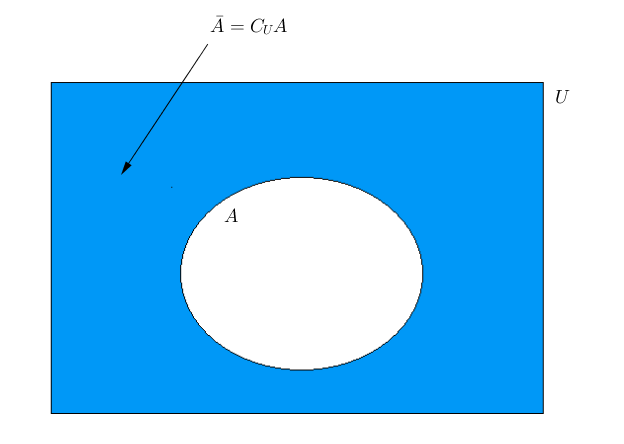
\includegraphics[scale=0.30]{Insiemi/venn-diagram2.png}
\end{center}

\subsection{Partizionamento di insiemi}
Sia \textit{F} un insieme i cui elementi sono insiemi, \textit{F} può essere anche chiamato \textbf{famiglia di insiemi}.
Dato un insieme non vuoto S, una \textbf{partizione} di S è una famiglia \textit{F} di sottoinsiemi di S tale che:
\begin{itemize}
    \item ogni elemento di S appartiene a qualche elemento di \textit{F}
    \item due elementi qualunque di \textit{F} sono disgiunti (intersezione vuota)
\end{itemize}